% !TEX program = xelatex

% Base
\documentclass{article}
\usepackage[a4paper,margin=1in]{geometry}

% Locale
\usepackage{polyglossia}
\setdefaultlanguage[localalph=true]{slovenian}
\usepackage[autostyle]{csquotes}
\DeclareQuoteAlias{german}{slovene}

% Bibliography
\usepackage[backend=biber,style=numeric]{biblatex}
\addbibresource{/home/martin/literatura.bib}

% Math
\usepackage{amsmath}
\usepackage{amssymb}
\usepackage{siunitx}
\usepackage{physics}

% Imported pdf_tex figures
\usepackage{graphicx,import}
\usepackage{subfig}
\usepackage{color}

% Hyperlinks
\usepackage{hyperref}
\usepackage[svgnames]{xcolor}

% Pgfplots
\usepackage{amssymb}

% Styling
\numberwithin{equation}{section}
\setlength{\skip\footins}{1.5cm}

% Differential
\newcommand{\diff}{\mathrm{d}}

% "Defined as" symbol
\usepackage{mathtools}
\newcommand{\das}{\vcentcolon=}
\newcommand{\asd}{=\vcentcolon}

\setcounter{page}{77}
\setcounter{section}{8}
\setcounter{subsection}{7}

\title{Poskusi z Rentgenskimi žarki}
\author{Martin Šifrar}

\begin{document}

%\maketitle

\subsection{Meritve}

Za napetosti na rentgenski cevi $\SI{15}{kv}$, $\SI{25}{kv}$, $\SI{30}{kv}$ in $\SI{30}{kv}$ pri toku $\SI{1}{mA}$ izmerimo odvisnosti ionizacijskega toka od napetosti na kondentzatorju $I_\mathrm{C}(U_\mathrm{C})$. Meritve so zapisane v tabeli~\ref{tab:I-by-U-data} in grafično prikazane na~\ref{fig:I-U}.

Izmerimo še, da ima ionizacijska celica (kondenzator) dimenzije

\begin{align*}
    a &= (160 \pm 0.5)\,\si{mm}, \\
    b &= \left( \frac{83+137}{2} \pm 0.5 \right)\,\si{mm}, \\
    c &= (34 \pm 0.5)\,\si{mm}.
\end{align*}

\begin{table}
    \centering
    \begin{tabular}{llll}
        \begin{tabular}{r|r}
            \multicolumn{2}{c}{$U_\mathrm{R} = \SI{15}{kV}$} \\
            \hline
            $U_\mathrm{C}\,[\si{V}]$ & $I_\mathrm{C}\,[\si{nA}]$ \\
            \hline
            0.0 & 0.02 \\
            9.7 & 0.08 \\
            21.2 & 0.12 \\
            29.8 & 0.14 \\
            39.3 & 0.15 \\
            48.7 & 0.16 \\
            59.1 & 0.15 \\
            69.5 & 0.16 \\
            80.6 & 0.16 \\
            90.5 & 0.16 \\
            101.4 & 0.17 \\
            120.7 & 0.15 \\
            148.2 & 0.17 \\
            178.7 & 0.18 \\
            206.5 & 0.16 \\
            253.2 & 0.17 \\
            300.9 & 0.18 \\
            & \\
            & \\
            & \\
            & \\
            & \\
        \end{tabular}
        &
        \begin{tabular}{r|r}
            \multicolumn{2}{c}{$U_\mathrm{R} = \SI{25}{kV}$} \\
            \hline
            $U_\mathrm{C}\,[\si{V}]$ & $I_\mathrm{C}\,[\si{nA}]$ \\
            \hline
            0.0 & 0.02 \\
            10.5 & 0.03 \\
            19.5 & 0.36 \\
            21.1 & 0.63 \\
            31.1 & 0.86 \\
            39.6 & 1.05 \\
            50.7 & 1.12 \\
            59.3 & 1.17 \\
            71.8 & 1.17 \\
            80.8 & 1.18 \\
            89.8 & 1.18 \\
            100.9 & 1.19 \\
            119.7 & 1.21 \\
            148.0 & 1.21 \\
            176.5 & 1.21 \\
            202.6 & 1.22 \\
            251.7 & 1.23 \\
            300.8 & 1.24 \\
            & \\
            & \\
            & \\
            & \\
        \end{tabular}
        &
        \begin{tabular}{r|r}
            \multicolumn{2}{c}{$U_\mathrm{R} = \SI{30}{kV}$} \\
            \hline
            $U_\mathrm{C}\,[\si{V}]$ & $I_\mathrm{C}\,[\si{nA}]$ \\
            \hline
            8.1 & 0.33 \\
            19.7 & 1.11 \\
            30.7 & 1.33 \\
            36.6 & 1.48 \\
            39.8 & 1.66 \\
            45.3 & 1.78 \\
            50.2 & 1.93 \\
            56.1 & 2.01 \\
            60.4 & 2.02 \\
            66.8 & 2.11 \\
            69.6 & 2.17 \\
            74.5 & 2.18 \\
            78.5 & 2.19 \\
            83.4 & 2.2 \\
            89.1 & 2.2 \\
            100.9 & 2.22 \\
            123.6 & 2.22 \\
            149.8 & 2.23 \\
            175.0 & 2.24 \\
            200.5 & 2.24 \\
            251.7 & 2.24 \\
            300.3 & 2.28 \\
        \end{tabular}
        &
        \begin{tabular}{r|r}
            \multicolumn{2}{c}{$U_\mathrm{R} = \SI{35}{kV}$} \\
            \hline
            $U_\mathrm{C}\,[\si{V}]$ & $I_\mathrm{C}\,[\si{nA}]$ \\
            \hline
            8.1 & 0.42 \\
            19.0 & 0.99 \\
            33.0 & 1.74 \\
            41.4 & 2.13 \\
            49.3 & 2.48 \\
            60.1 & 2.87 \\
            69.8 & 3.09 \\
            79.7 & 3.24 \\
            91.3 & 3.34 \\
            100.5 & 3.45 \\
            117.9 & 3.49 \\
            150.3 & 3.51 \\
            173.7 & 3.53 \\
            201.2 & 3.54 \\
            249.1 & 3.54 \\
            299.2 & 3.59 \\
            & \\
            & \\
            & \\
            & \\
            & \\
            & \\
        \end{tabular}
    \end{tabular}
    \caption{Meritve ionizacijskega toka v odvisnosti od napetosti na kondenzatorju.}
    \label{tab:I-by-U-data}
\end{table}

Za meritev\footnote{Meritev polarizacije nisem izvajal sam, saj je GM števec pri vaji trenutno pokvarjen. Uporabil sem meritve iz prejšnjih let. Avtor teh meritev ni zapisal napak samih meritev, le simbolen izračun napake in napako končnega rezultata, torej te meritve nimajo napak.} polarizacije primarnih žarkov s sipanjem izmerimo intenzitete

\begin{align}
    I_z &= 115\,\si{s^{-1}}, \\
    I_{z0} &= 0.25\,\si{s^{-1}}, \\
    I_{x} &= 133.2\,\si{s^{-1}}, \\
    I_{x0} &= 0.25\,\si{s^{-1}},
    \label{eq:polar-1}
\end{align}

pri čemer so intenzitete z indeksi 0 ozadja, ki jih kasneje od pripadajoče meritve odštejemo. Za meritev polarizacije že sipanih žarkov pa

\begin{align}
    I_z &= 0.40\,\si{s^{-1}}, \\
    I_{z0} &= 0.35\,\si{s^{-1}}, \\
    I_{y} &= 0.38\,\si{s^{-1}}, \\
    I_{y0} &= 0.28\,\si{s^{-1}}.
    \label{eq:polar-2}
\end{align}

\begin{figure}
    \begin{center}
        \includegraphics{I-by-U.pdf}
    \end{center}
    \caption{Izmerjene vrednosti toka $I_\mathrm{C}$ med ploščama kondenzatorja za različne napetosti na kondenzatorju. Odvisnost je izmerjena za 4 različne napetosti na rentgenski cevi; tok na rentgenski cevi pa je konstanten, sicer $1\,\mathrm{mA}$. Črte, ki povezujejo meritve, so zgolj z a boljšo preglednost.}
    \label{fig:I-U}
\end{figure}

\begin{figure}
    \begin{center}
        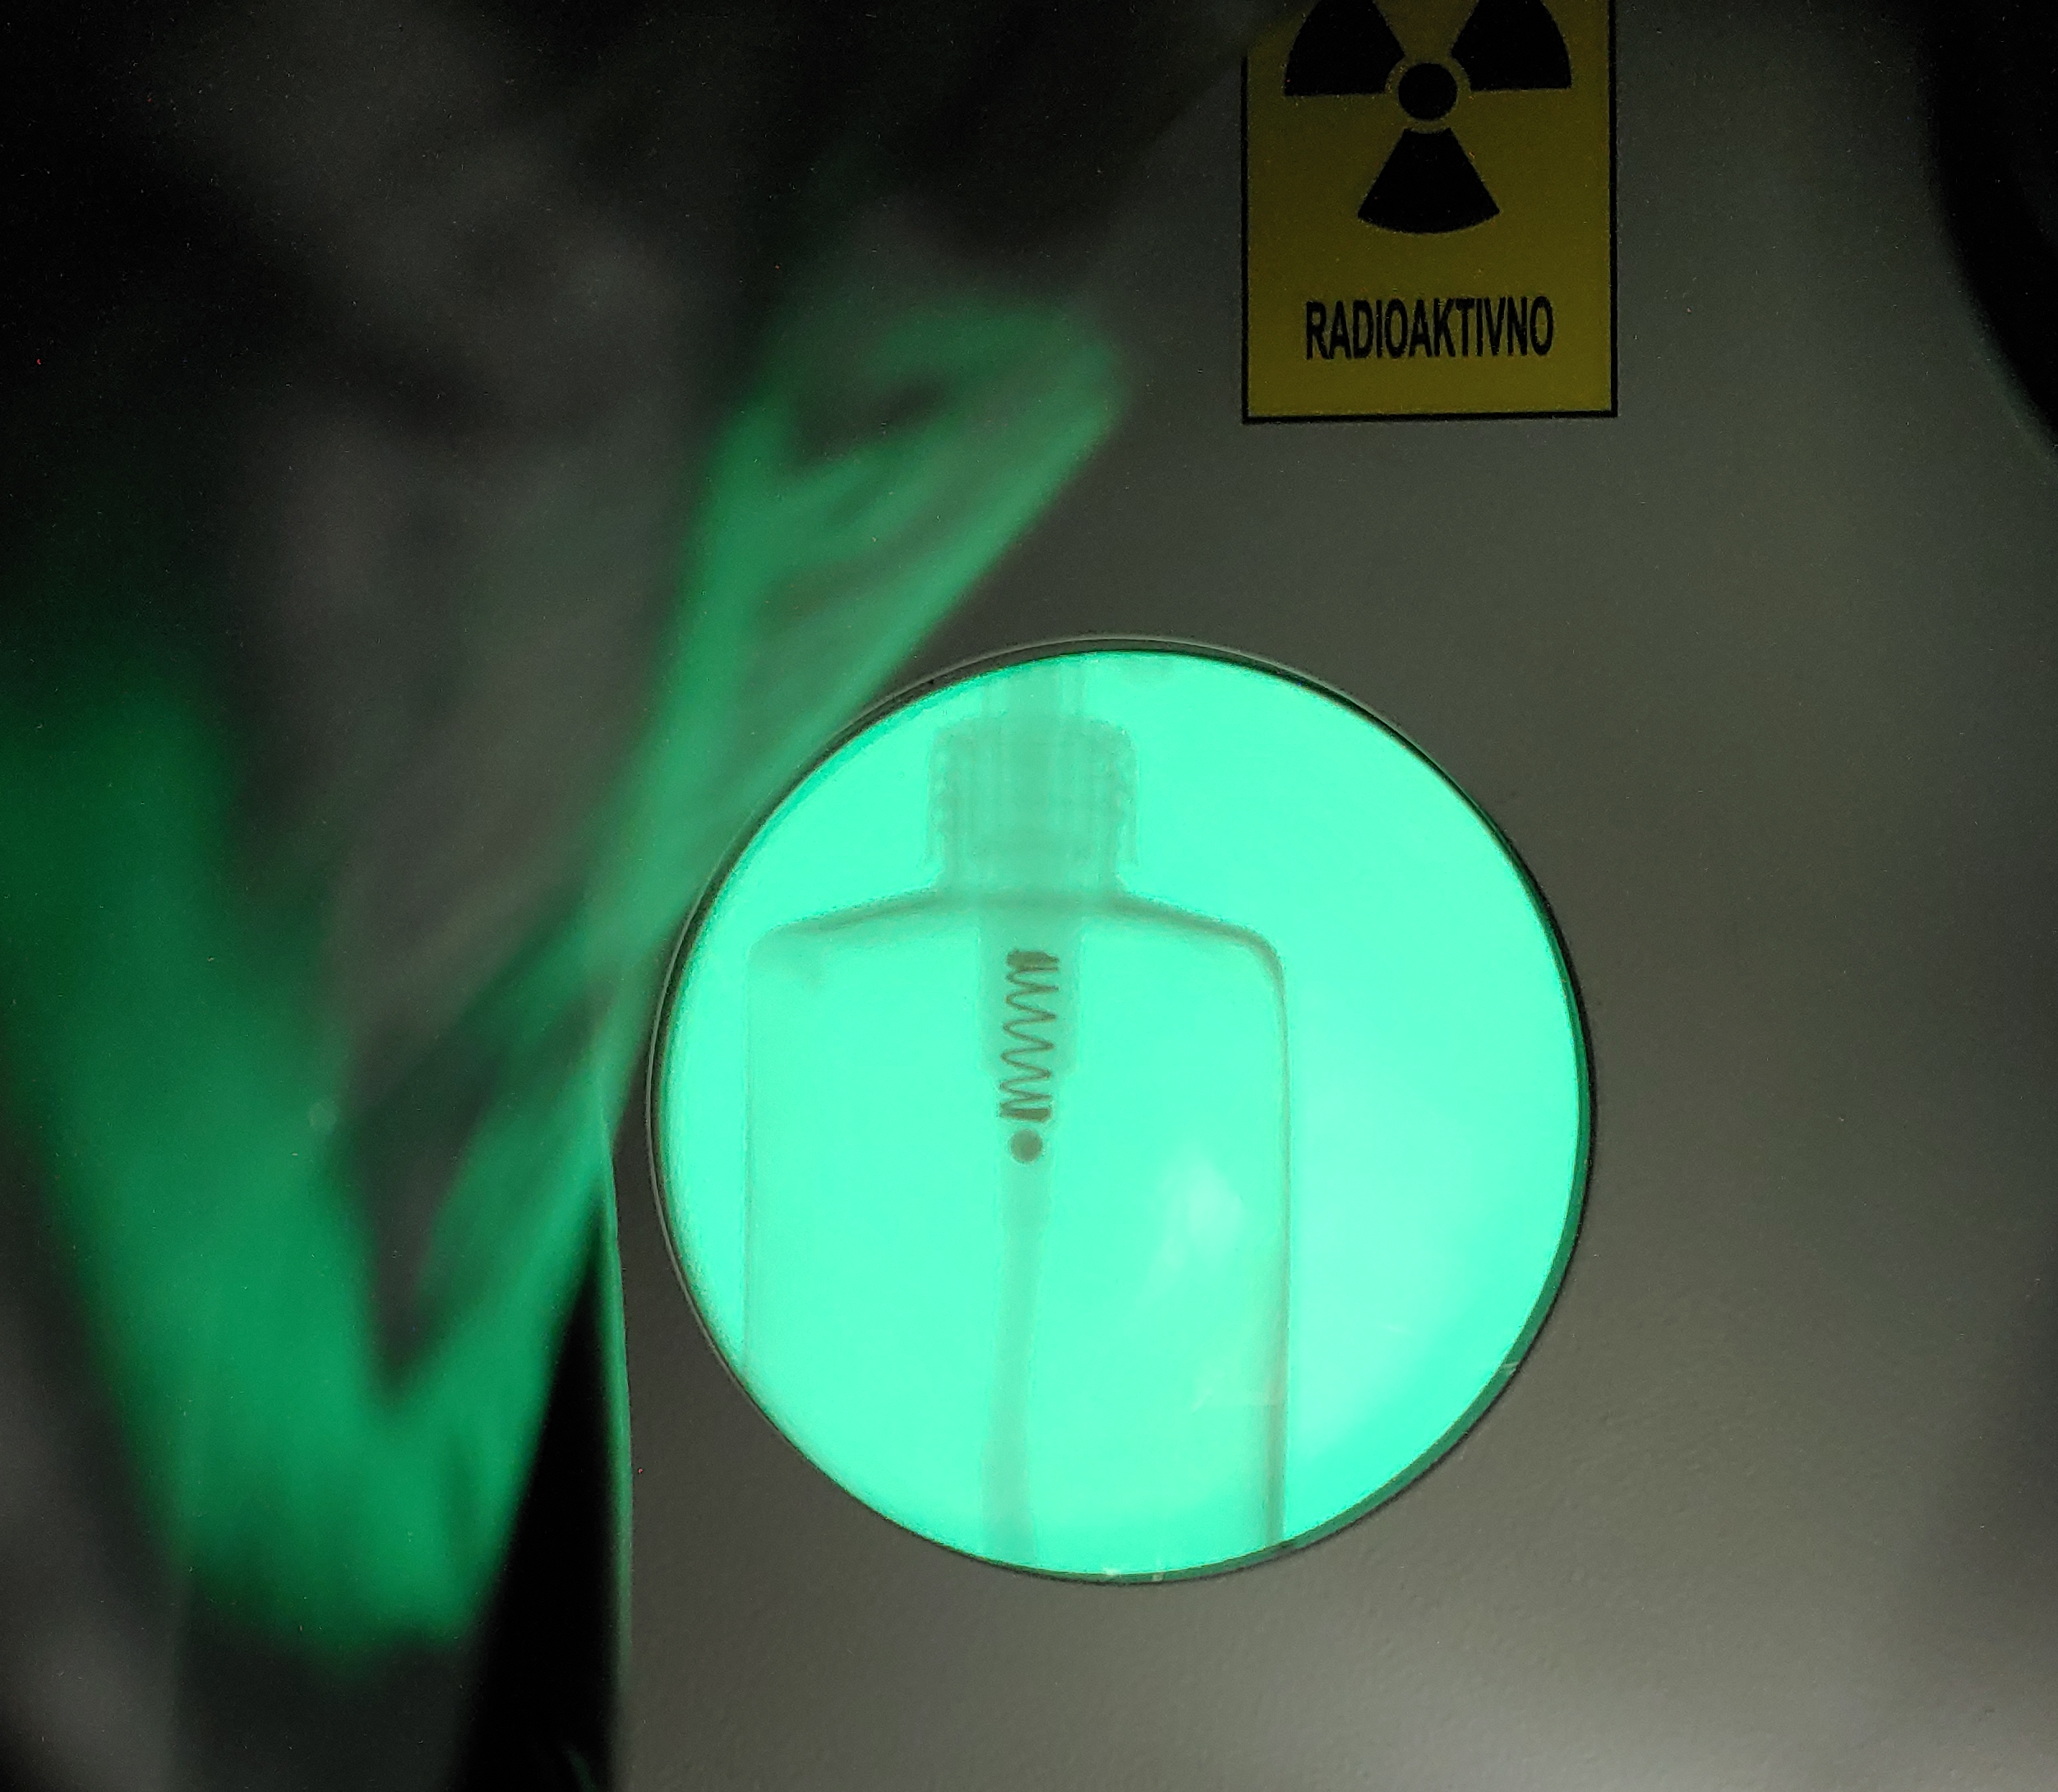
\includegraphics[width=0.65\textwidth]{sanitizer.png}
    \end{center}
    \caption{Rentgenski posnetkek dispenzerja za razkužilo.}
    \label{fig:sanitizer}
\end{figure}

\begin{figure}
    \begin{center}
        \includegraphics[width=\textwidth]{stopwatch-powerbrick.png}
    \end{center}
    \caption{Rentgenska posnetka štoparice in polnilca za telefon.}
    \label{fig:stopwatch-powerbrick}
\end{figure}

\subsection{Račun}

Za volumen ionizacijske celice iz meritev izračunamo

\begin{equation*}
    V = 600\,(1 \pm 0.02)\,\si{mm^3}.
\end{equation*}

Iz meritev na sliki~\ref{fig:I-U}, posebej na sliki~\ref{fig:I-U-saturated} izračunamo nasičene ionizacijske tokove $I_\mathrm{nasičen}$ (vrednosti v tabeli~\ref{tab:I-saturated}). Hitrost doze lahko potem izračunamo z izrazom

\begin{equation*}
    \dot{X} = \frac{I_\mathrm{nasičen}}{\rho V},
\end{equation*}

kjer za $\rho$ uporabimo gostoto zraka

\begin{equation*}
    \rho = \SI{1.204}{kg/m^3}.
\end{equation*}

Izračunane hitrosti doze predstavimo v tabeli~\ref{tab:I-saturated}.

\begin{table}
    \centering
    \begin{tabular}{r|r r}
        $U_\mathrm{R}\,[\si{kV}]$ & $I_\mathrm{nasičen}\,[\si{nA}]$ & $\dot{X}\,[\si{mAs/kg h}]$ \\
        \hline
        15 & $0.17 \pm 0.01$ & $0.83 \pm 0.07$ \\
        25 & $1.20 \pm 0.02$ & $6.0 \pm 0.2$ \\
        30 & $2.23 \pm 0.03$ & $11.1 \pm 0.4$ \\
        35 & $3.52 \pm 0.04$ & $17.6 \pm 0.6$ \\
    \end{tabular}
    \caption{Iz napetostnega intervala $U_\mathrm{C} \in [100, 300]$ izračunane vrednosti zasičenega toka $I_\mathrm{C}$. Primerjamo jih lahko s prikazom meritev na sliki~\ref{fig:I-U-saturated}.}
    \label{tab:I-saturated}
\end{table}

\begin{figure}
    \begin{center}
        \includegraphics{I-by-U-saturated.pdf}
    \end{center}
    \caption{Prikaz meritev iz~\ref{fig:I-U}, iz katere lažje razberemo zasičen tok $U_\mathrm{C}$.}
    \label{fig:I-U-saturated}
\end{figure}

Iz meritev~\ref{eq:polar-1} za polarizacijo primarnih žarkov lahko polarizacijo izračunamo preko

\begin{equation*}
    \eta = \frac{I_z - I_x}{I_z + I_x}.
\end{equation*}

Za polarizacijo izračunamo\footnote{Glej opombo 1.} vrednost

\begin{equation*}
    \eta = 0.07 \pm 0.01.
\end{equation*}

Polarizacijo že sipanih žarkov izračunamo podobno, le da tokrat gledamo ravnino $xy$ namesto ravnine $xz$. Izračunamo\footnote{Glej opombo 1} polarizacijo

\begin{equation*}
    \eta = 0.33 \pm 0.15.
\end{equation*}

\end{document}
